%%%%%%%%%%%%%%%%%%%%%%%%%%%%%%%%%%%%%%%%%%%%%%%%%%%%%%%%%%%

\section{Apresentação dos dados}

A base de dados BloodMNIST é formada por um total de 15380 imagens de células sanguíneas divdidas em 8 classes, como mostrado na \autoref{fig:samples_of_classes}. Essas amostras se dividem em conjunto de treinamento, com 11959 representantes e teste, com 3421 itens. As imagens estão disponíveis em diferentes resoluções, sendo \textit{a priori}, escolhida a resolução de 28x28 para trazer mais eficiência computacional, principalmente para o caso das redes densas. Porém, propõem-se o teste de amostras de maior resolução para a rede convolucional já treinada com as amostras 28x28, para validação da robustez ao tamanho da entrada.

\begin{figure}[H]
	\centering
	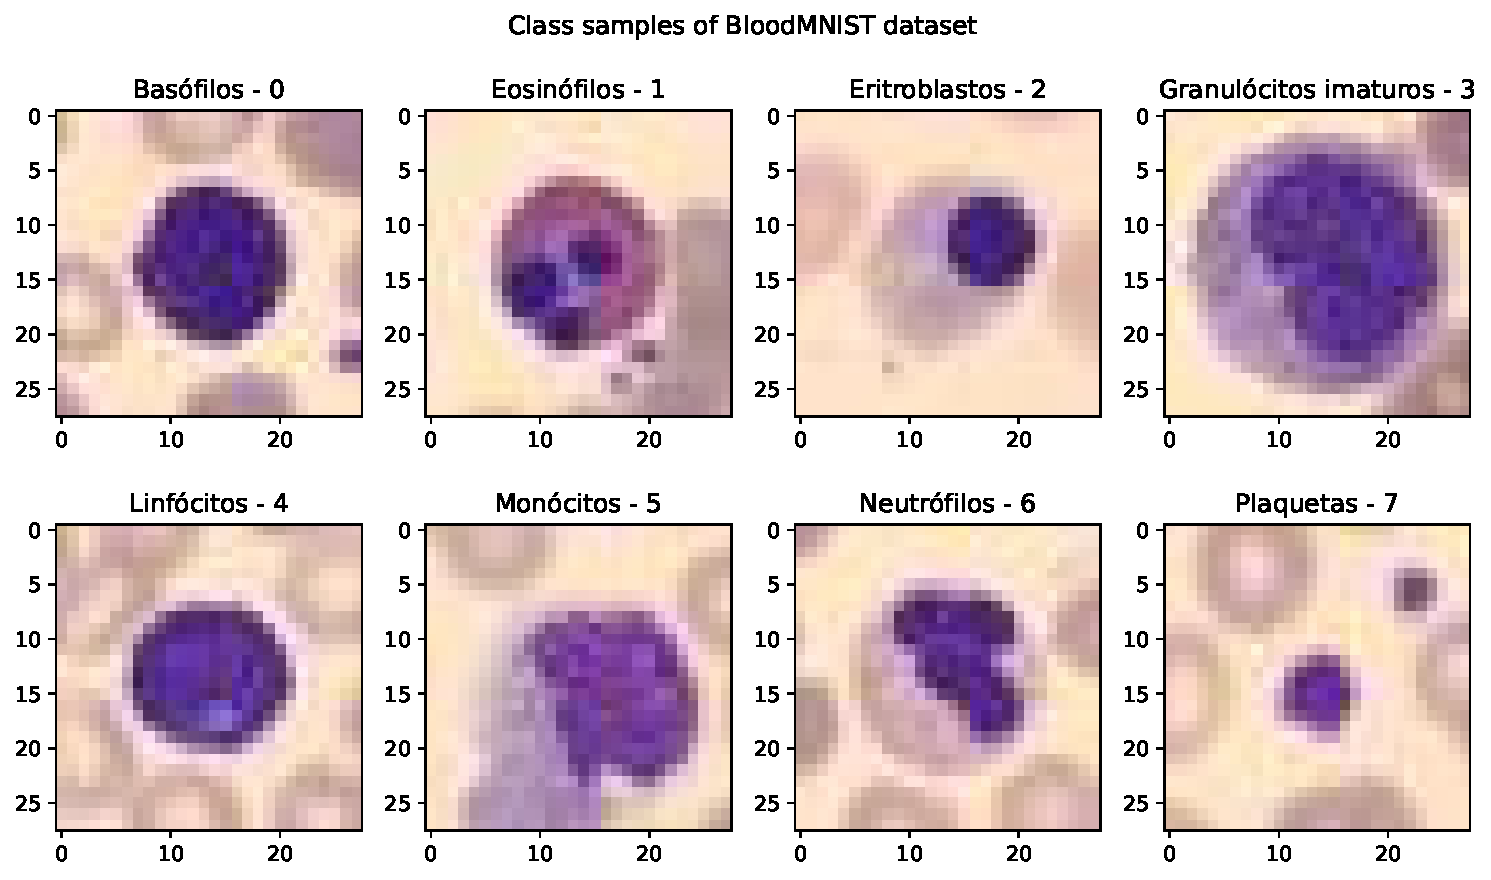
\includegraphics[width=0.75\linewidth]{../../plot/samples_of_classes}
	\caption{Amostras das classes do \textit{dataset} BloodMNIST.}
	\label{fig:samples_of_classes}
\end{figure}

O \textit{dataset} BloodMNIST já fornece de forma separada os dados utilizados para treinamento, e os que serão utilizados para teste. A \autoref{fig:balancingofclasses} mostra a distribuição de amostrar para cada classe, para os conjuntos de treinamento, em azul, e de teste, em verde. Observa-se que existem classes majoritárias, como a 1, 3, 6 e 7, que apresentam muito mais amostras que as demais. O perfil de amostras por classe é similar nos conjuntos de teste e treinamento, o que mostra que o impacto no mapeamento pelo desbalanceamento das classes irá afetar de forma igual ambos os \textit{datasets}. \textbf{Tal disparidade pode ser tanto causada por um viés na coleta de dados, quanto também pela ocorrência real de mais representantes de uma classe do que das demais, o que modela de forma realista os dados.}

% TODO: \usepackage{graphicx} required
\begin{figure}[H]
	\centering
	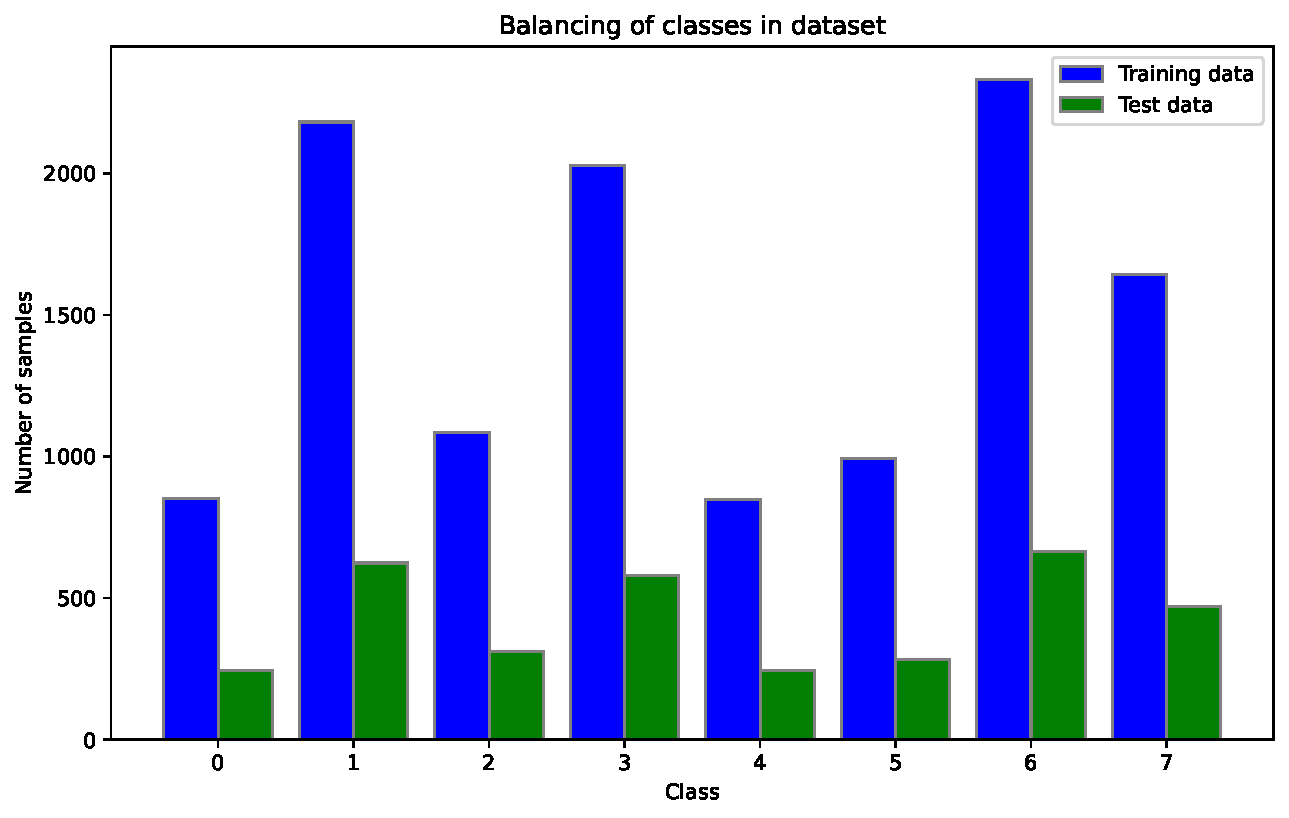
\includegraphics[width=0.75\linewidth]{../../plot/Balancing_of_classes}
	\caption{Balanço das classes nos \textit{datasets} de treinamento e teste.}
	\label{fig:balancingofclasses}
\end{figure}

Para realizar o treinamento utilizando da ferramenta de validação cruzada, foi escolhida a validação do tipo \textit{holdout}, por meio do particionamento do conjunto de dados de treinamento, obtendo um novo conjunto de dados de validação. O novo conjunto de treinamento é formado pelos primeiros 70\% do conjunto original de treinamento, enquanto o de validação, os 30\% restantes do final do \textit{dataset} original. Para garantir a veracidade da validação, quer-se que ambos os conjuntos tenham a mesma representação de cada classe, o que pode se afirmar positivo de acordo com a \autoref{fig:balancingofclasses_holdout}.

% TODO: \usepackage{graphicx} required
\begin{figure}[H]
\centering
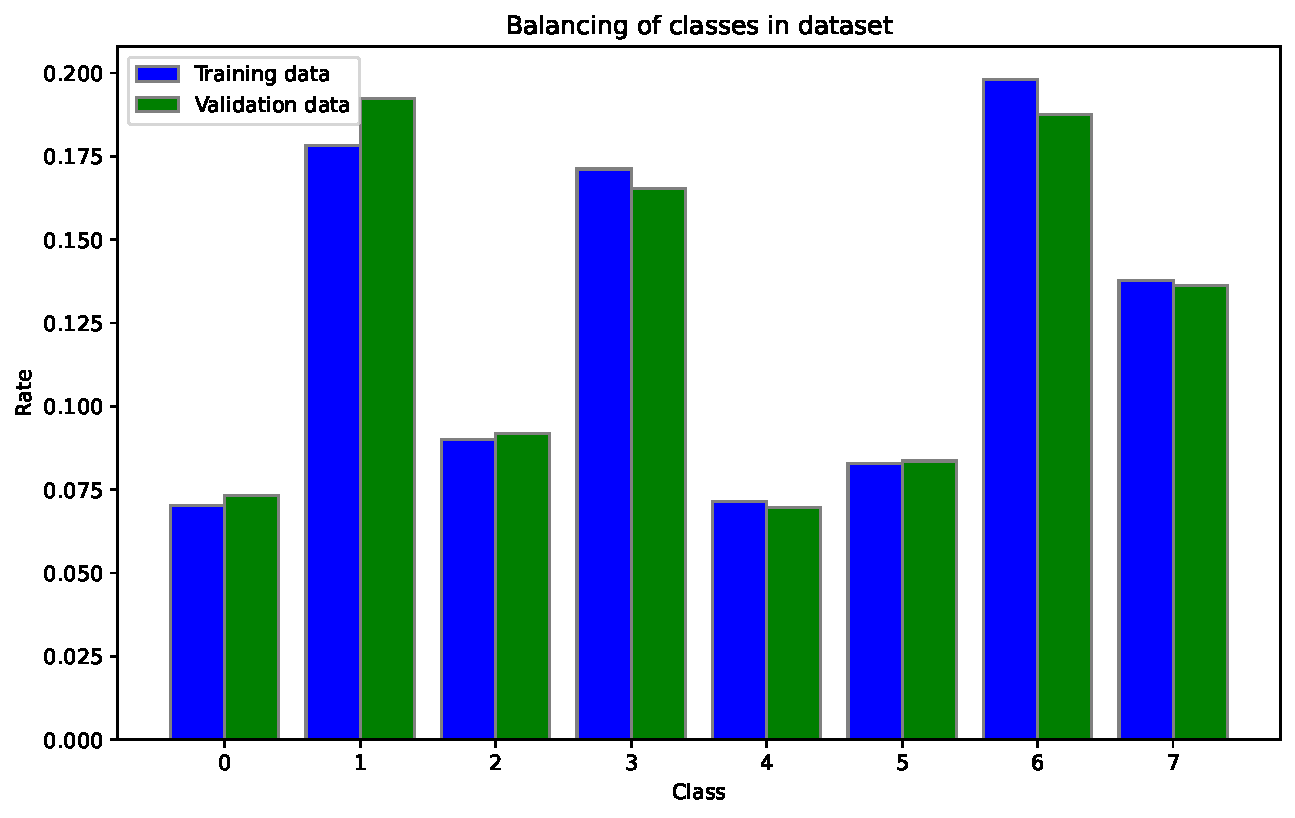
\includegraphics[width=0.75\linewidth]{../../plot/Balancing_of_classes_holdout}
\caption{Balanço das classes nos conjuntos de dados de treinamento e validação cruzada do tipo \textit{holdout}.}
\label{fig:balancingofclasses_holdout}
\end{figure}


\section{MLP}

A implementação da rede MLP com uma camada intermediária se deu por meio do uso do \textit{framework} TensorFlow, possuindo uma camada de entrada que sequencia os pixels da imagem em um vetor, uma camada de neurônios intermediária, e uma camada de saída com função de ativação \textit{softmax} para geração do vetor \textit{one-hot encoding} das probabilidades da entrada pertencer à cada uma das 8 classes.

\subsection{Busca do melhor modelo}

Para realizar a busca do melhor modelo da MLP, considerando que existem uma grande possibilidade de hiper-parâmetros, foi realizada uma busca exaustiva simplificada por etapas, baseada no funcionamento dos \textit{wrappers}, onde dada uma configuração inicial de parâmetros, baseado no comumente visto na literatura \cite{geron2019hands}. As variáveis selecionadas para a busca foram: Número de neurônios da camada intermediária, função de ativação dos neurônios da camada intermediária, taxa de \textit{dropout} dos neurônios da camada intermediária e otimizador para ajuste dos pesos. Demais hiper-parâmetros como tamanho do \textit{batch} e passo do algoritmo de otimização foram mantidos \textit{default}.

A busca por etapas se deu da seguinte forma: Dada a condição inicial, uma MLP de 256 neurônios na camada intermediária com função de ativação ReLU, sem \textit{dropout} e ajustada por \textit{Stochastic Gradient Descendent} (SGD), testou-se a rede alterando primeiramente o número de neurônios. Uma vez conhecido o valor que obteve maior acurácia, testou-se as funções de ativações canditadas para esse número de neurônios, buscando a combinação que desse a melhor acurácia. O processo se repete para o \textit{dropout} e o algoritmo de otimização, onde ao final se obtém a combinação que agrega o melhor número de neurônios visto, melhor função de ativação para tal conjunto de neurônios, melhor taxa de \textit{dropout} e o melhor otimizador.


\begin{itemize}
	\item Número de neurônios: [ \texttt{256}, \texttt{512}, \texttt{1024}, \texttt{2048}, \texttt{4096} ]
	\item Função de ativação: [ \texttt{ReLU}, \texttt{Sigmoide} ]
	\item \textit{Dropout}: [ \texttt{0,0}, \texttt{0,25}, \texttt{0,5} ]
	\item Otimizador: [ \texttt{SGD}, \texttt{ADAM} ]
\end{itemize} 

\subsubsection{Número de neurônios}

\begin{figure}[H]
	\centering
	\begin{subfigure}[H]{0.49\textwidth}
		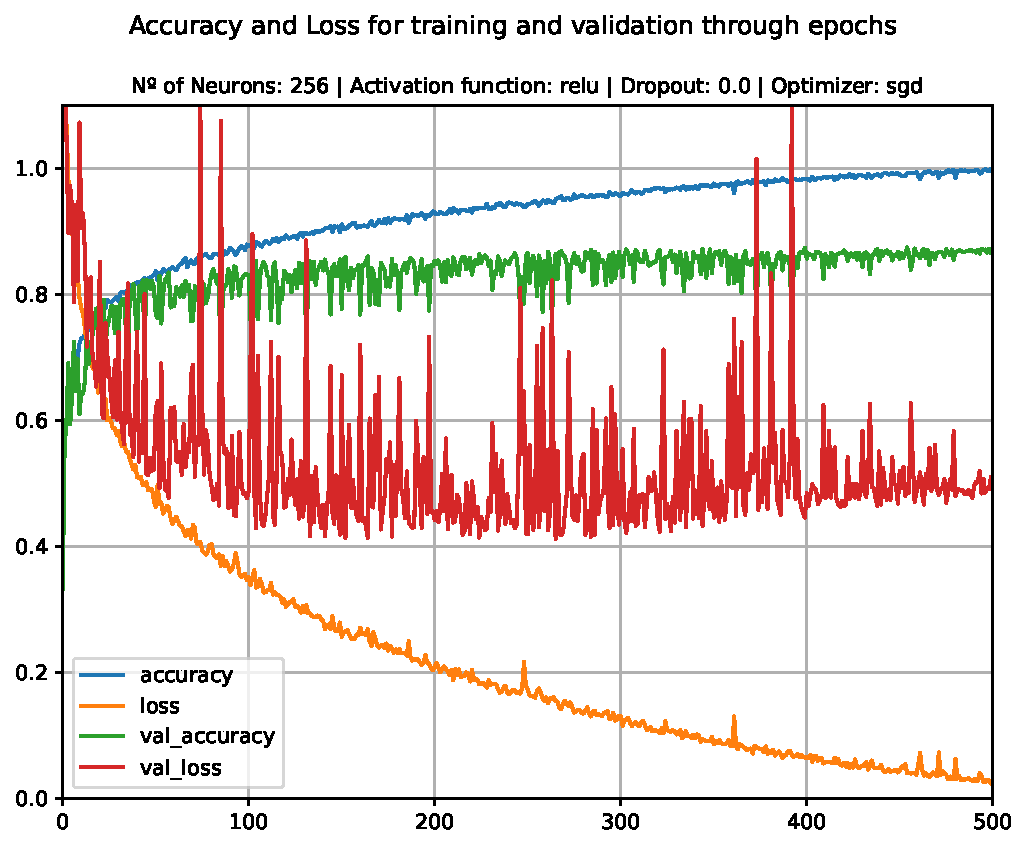
\includegraphics[width = \textwidth]{../../plot/mlp/mlp_256_relu_0.0_sgd}
		\caption{256 neurônios.}
		\label{fig:mlp_256_relu_0.0_sgd}
	\end{subfigure}
	\begin{subfigure}[H]{0.49\textwidth}
		\centering
		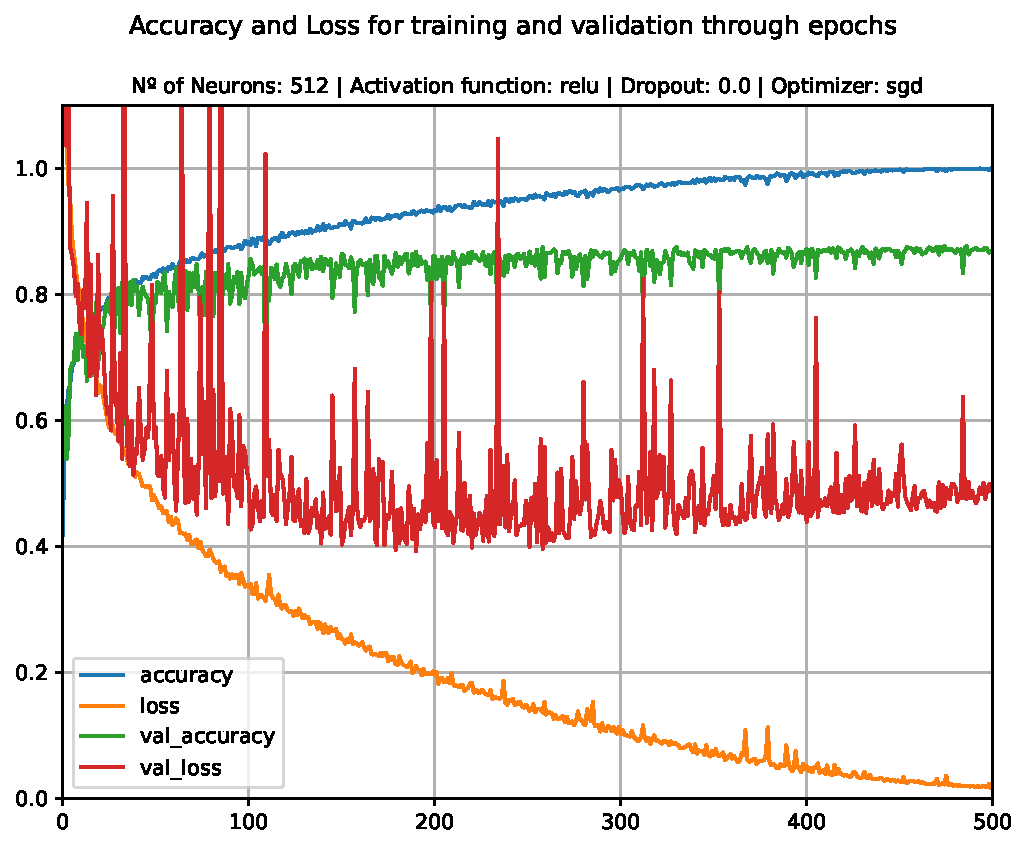
\includegraphics[width = \textwidth]{../../plot/mlp/mlp_512_relu_0.0_sgd}
		\caption{512 neurônios.}
		\label{fig:mlp_512_relu_0.0_sgd}
	\end{subfigure}
	\begin{subfigure}[H]{0.49\textwidth}
		\centering
		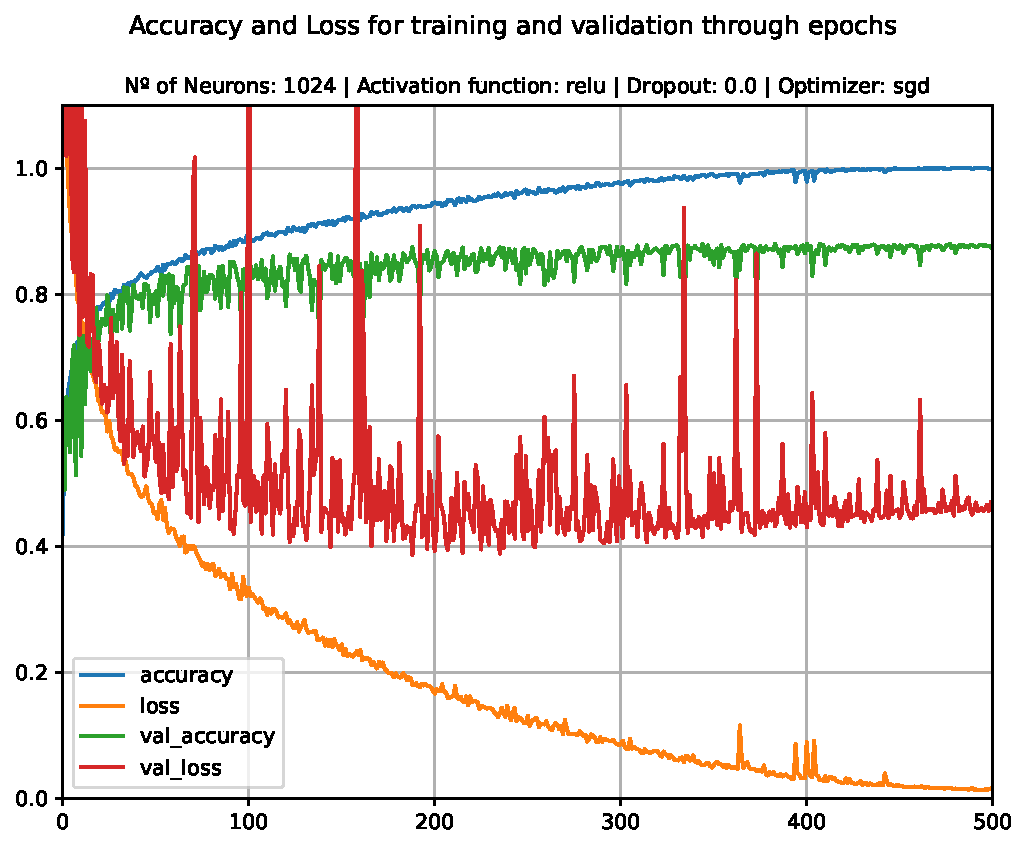
\includegraphics[width = \textwidth]{../../plot/mlp/mlp_1024_relu_0.0_sgd}
		\caption{1024 neurônios.}
		\label{fig:mlp_1024_relu_0.0_sgd}
	\end{subfigure}
	\begin{subfigure}[H]{0.49\textwidth}
		\centering
		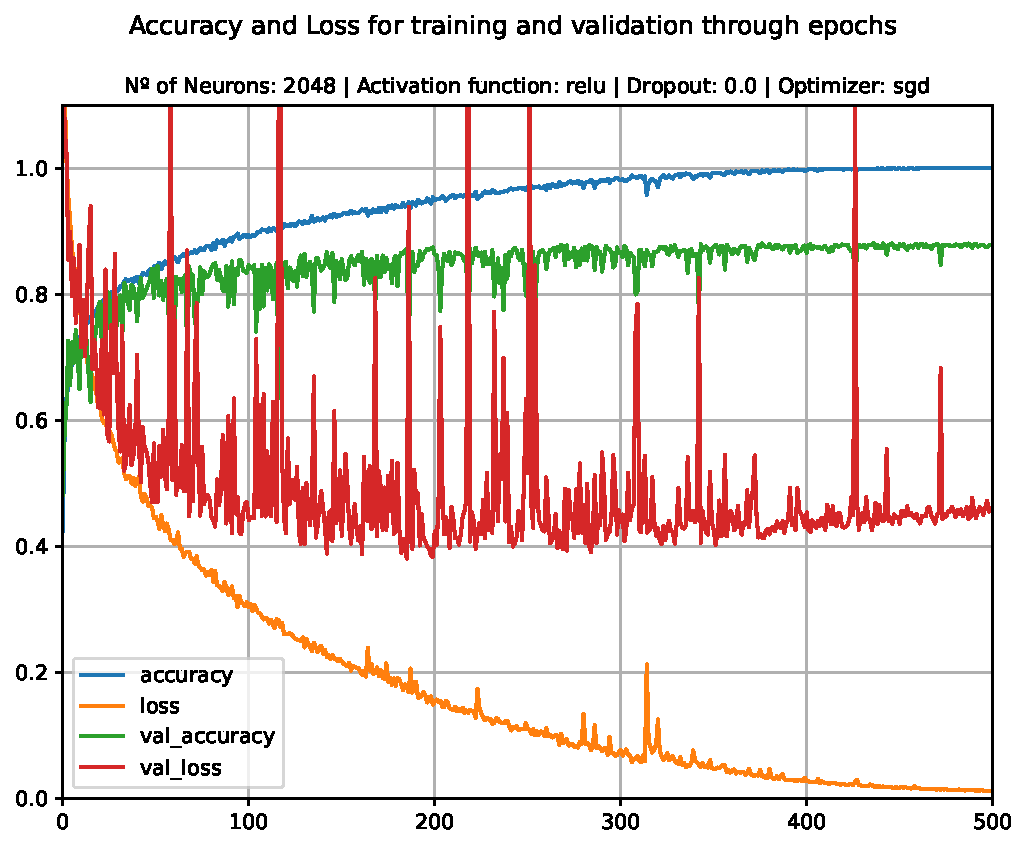
\includegraphics[width = \textwidth]{../../plot/mlp/mlp_2048_relu_0.0_sgd}
		\caption{2048 neurônios.}
		\label{fig:mlp_2048_relu_0.0_sgd}
	\end{subfigure}
	\begin{subfigure}[H]{0.49\textwidth}
		\centering
		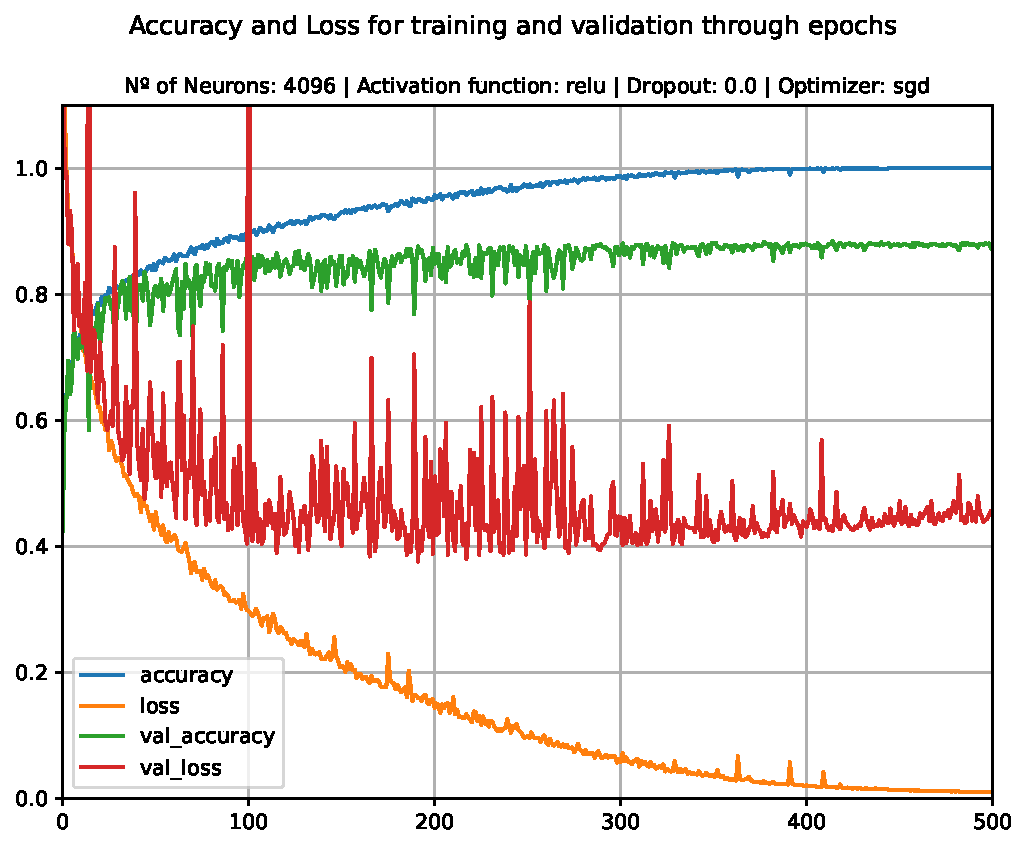
\includegraphics[width = \textwidth]{../../plot/mlp/mlp_4096_relu_0.0_sgd}
		\caption{4096 neurônios.}
		\label{fig:mlp_4096_relu_0.0_sgd}
	\end{subfigure}
	\caption{Evolução da perda e acurácia de treinamento e validação com as épocas de treinamento para cada número de neurônios avaliados.}
\end{figure}


\begin{figure}[H]
	\centering
	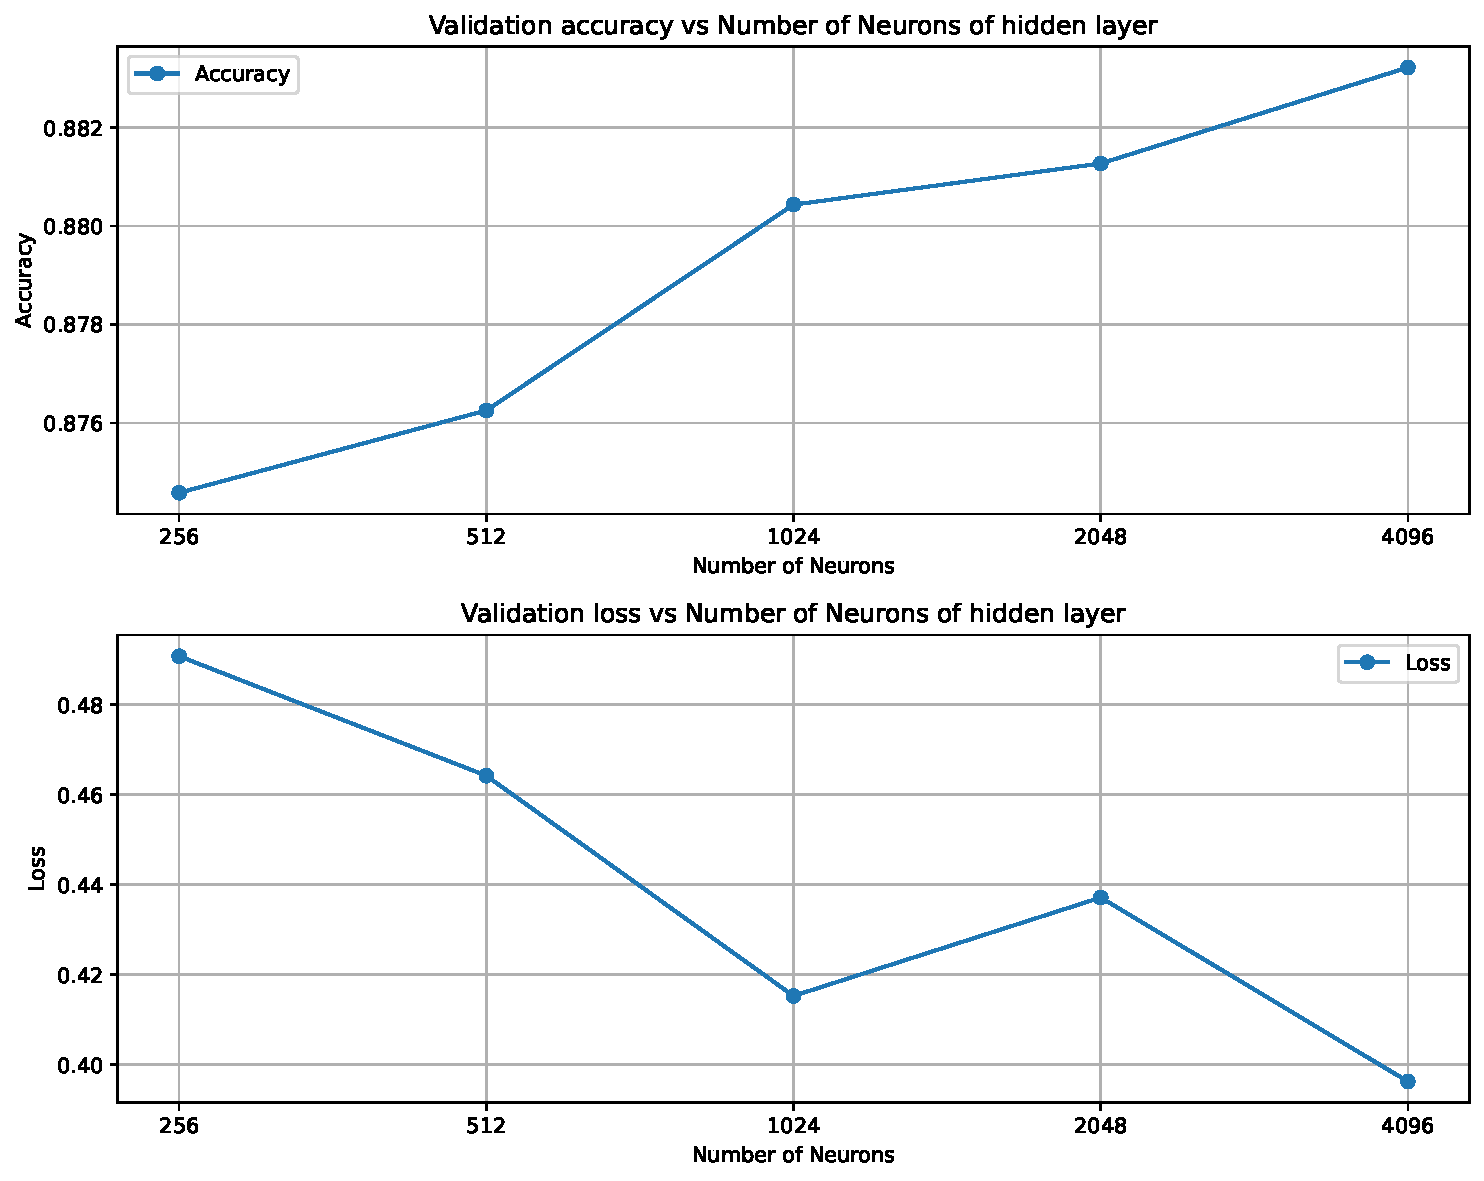
\includegraphics[width=0.75\linewidth]{../../plot/mlp/search_neurons}
	\caption{Acurácia e perda com a variação do número de neurônios da camada intermediária.}
	\label{fig:search_neurons}
\end{figure}

\subsubsection{Função de ativação}

\begin{figure}[H]
	\centering
	\begin{subfigure}[H]{0.49\textwidth}
		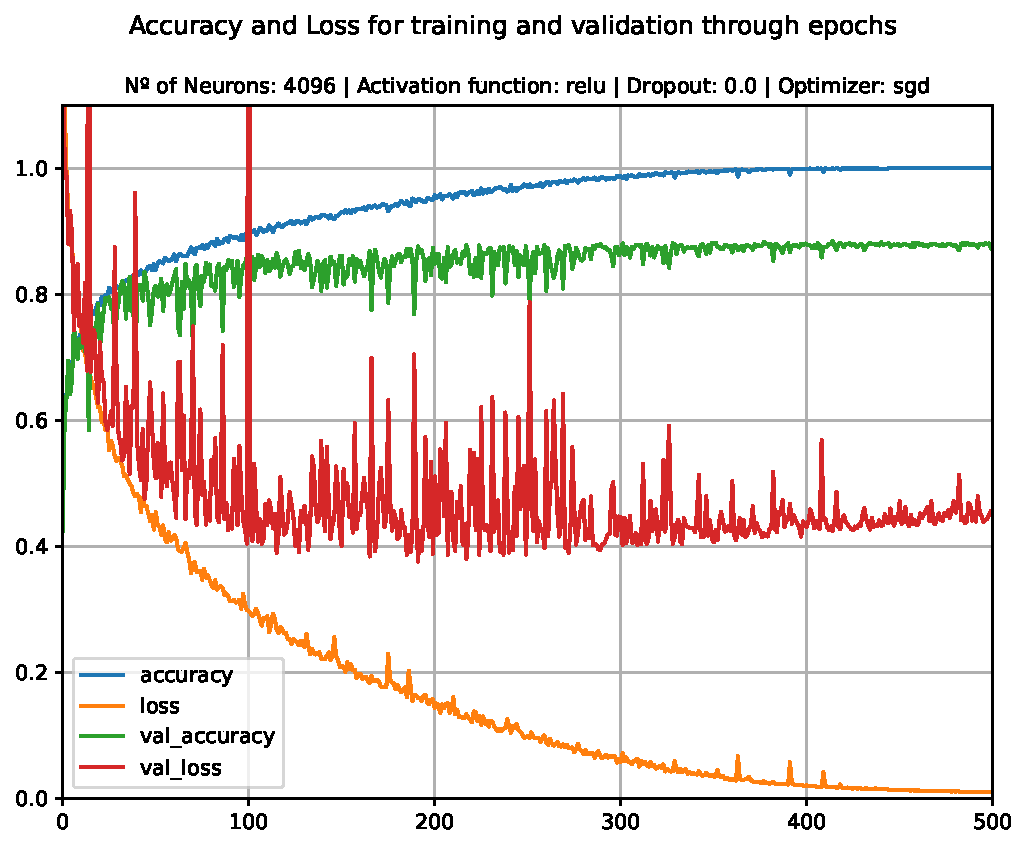
\includegraphics[width = \textwidth]{../../plot/mlp/mlp_4096_relu_0.0_sgd}
		\caption{ReLU.}
		\label{fig:mlp_4096_relu_0.0_sgd_act_fnc}
	\end{subfigure}
	\begin{subfigure}[H]{0.49\textwidth}
		\centering
		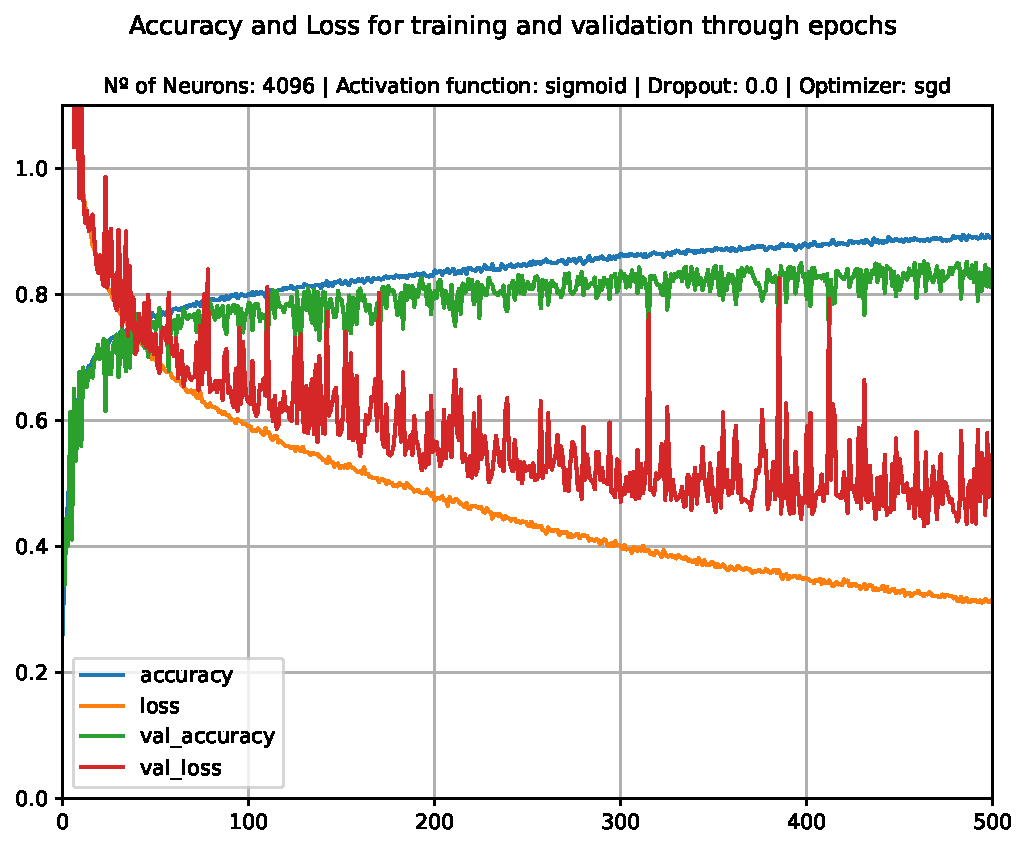
\includegraphics[width = \textwidth]{../../plot/mlp/mlp_4096_sigmoid_0.0_sgd}
		\caption{Sigmoide.}
		\label{fig:mlp_4096_sigmoid_0.0_sgd}
	\end{subfigure}
	\caption{Evolução da perda e acurácia de treinamento e validação com as épocas de treinamento para cada função de ativação candidata.}
\end{figure}

\begin{figure}[H]
\centering
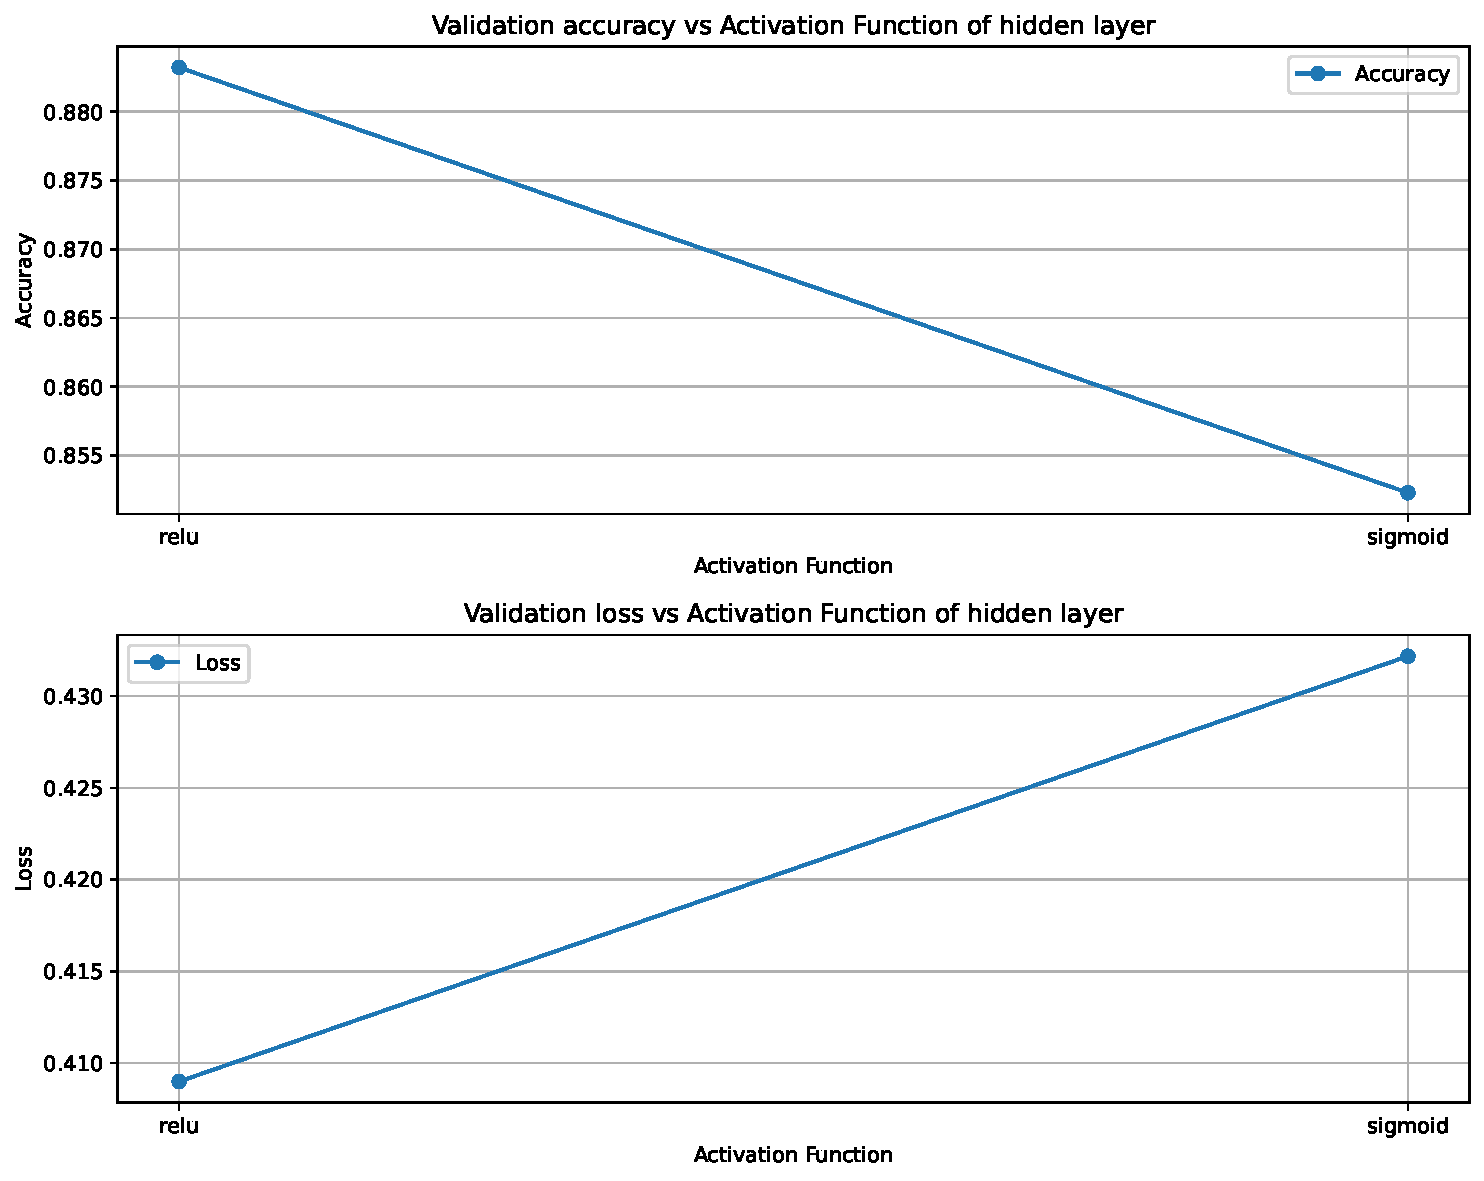
\includegraphics[width=0.75\linewidth]{../../plot/mlp/search_activation_fnc}
\caption{Acurácia e perda com a variação da função de ativação dos neurônios da camada intermediária.}
\label{fig:search_activation_fnc}
\end{figure}

\subsubsection{\textit{Dropout}}

\begin{figure}[H]
	\centering
	\begin{subfigure}[H]{0.49\textwidth}
		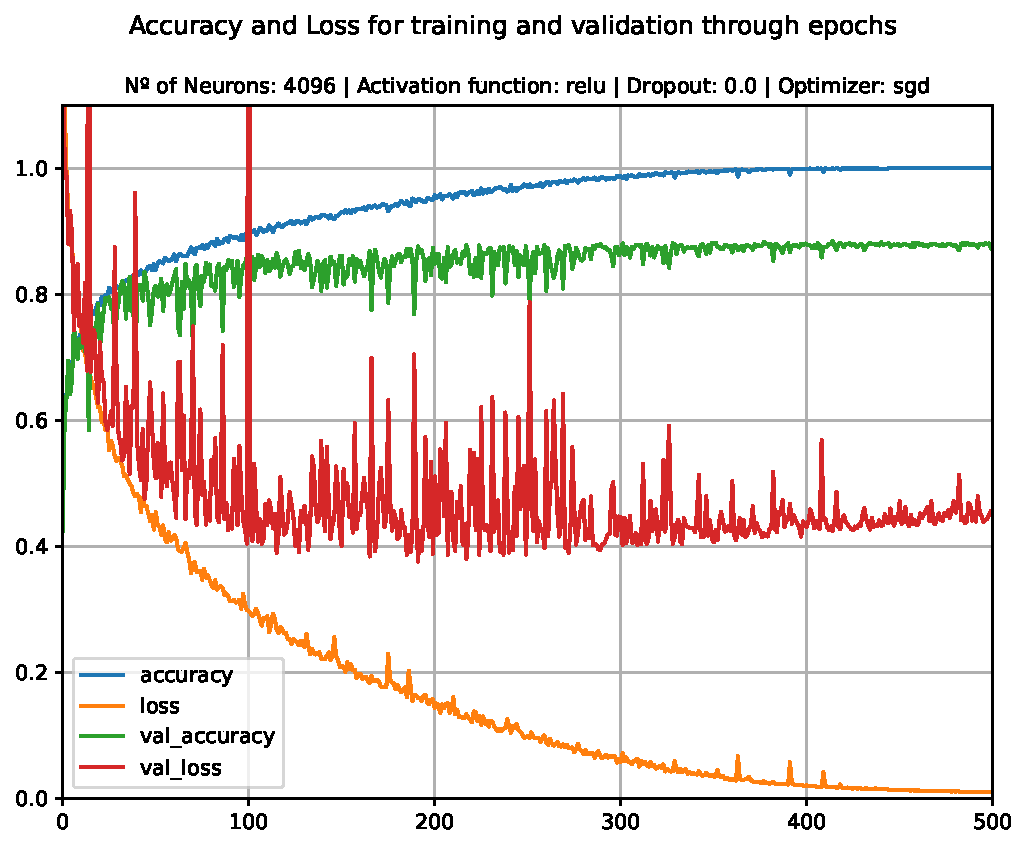
\includegraphics[width = \textwidth]{../../plot/mlp/mlp_4096_relu_0.0_sgd}
		\caption{0,0.}
		\label{fig:mlp_4096_relu_0.0_sgd_dropout}
	\end{subfigure}
	\begin{subfigure}[H]{0.49\textwidth}
		\centering
		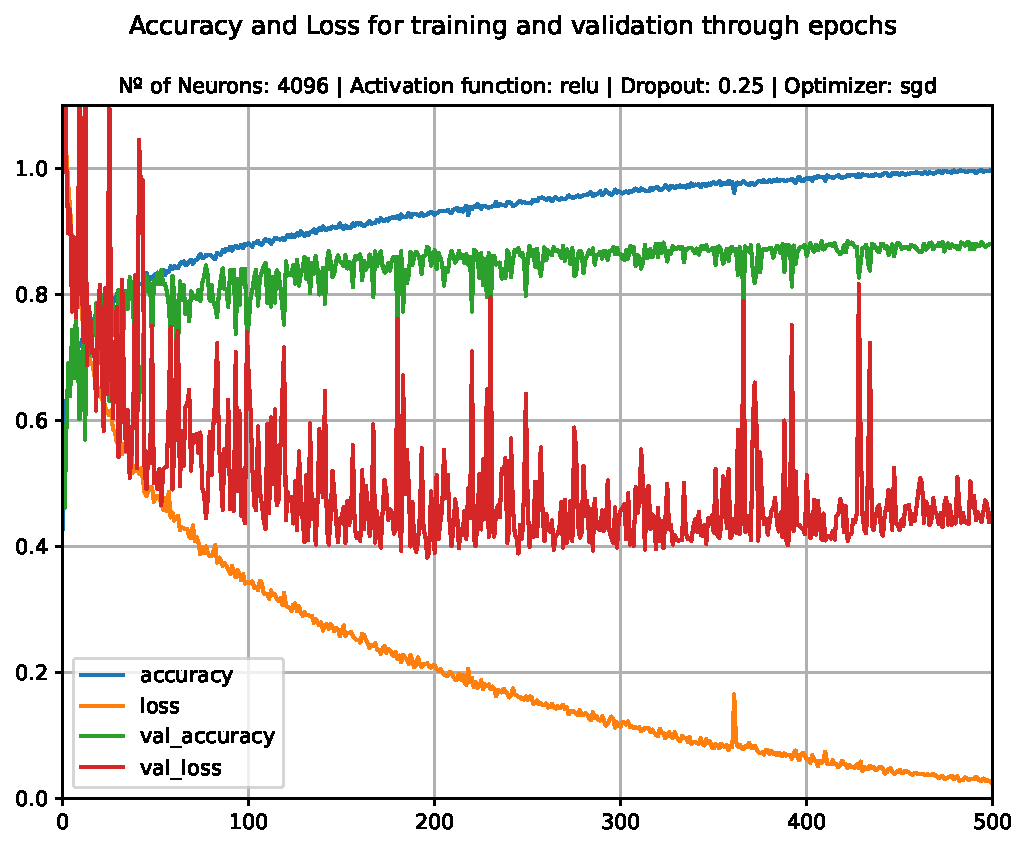
\includegraphics[width = \textwidth]{../../plot/mlp/mlp_4096_relu_0.25_sgd}
		\caption{0,25.}
		\label{fig:mlp_4096_relu_0.25_sgd}
	\end{subfigure}
	\begin{subfigure}[H]{0.49\textwidth}
		\centering
		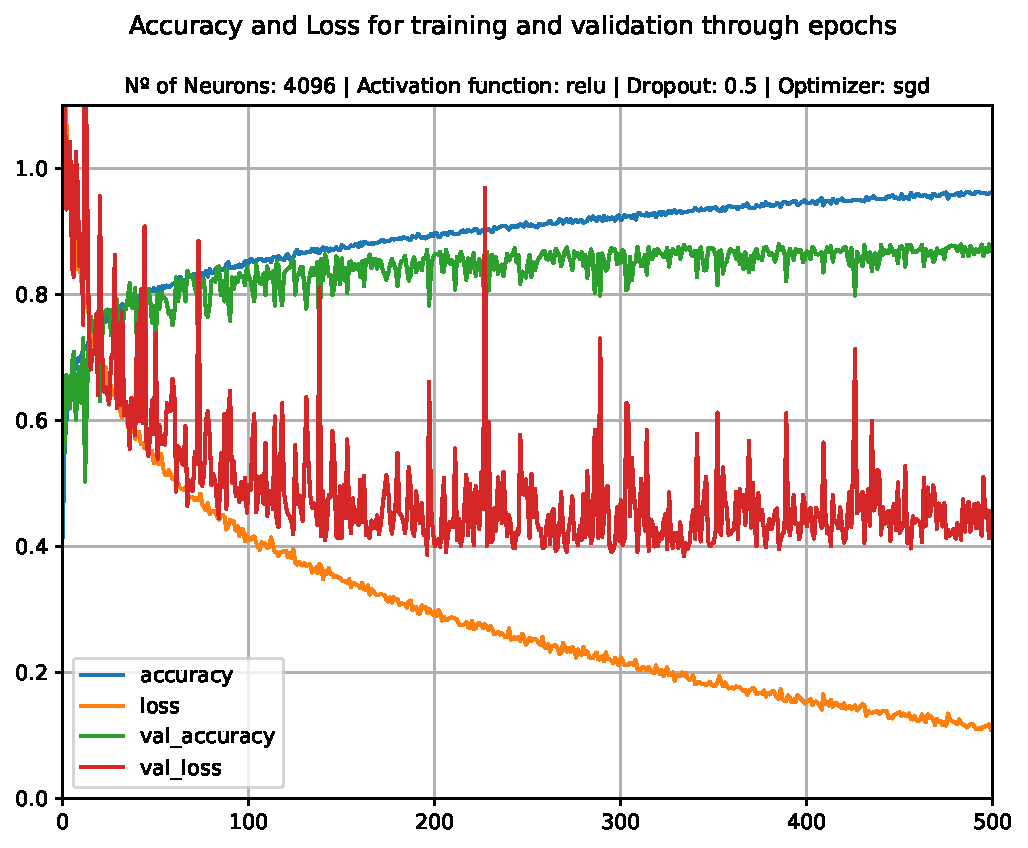
\includegraphics[width = \textwidth]{../../plot/mlp/mlp_4096_relu_0.5_sgd}
		\caption{0,5.}
		\label{fig:mlp_4096_relu_0.5_sgd}
	\end{subfigure}
	\caption{Evolução da perda e acurácia de treinamento e validação com as épocas de treinamento para diferentes taxas de \textit{dropout}.}
\end{figure}

\begin{figure}[H]
\centering
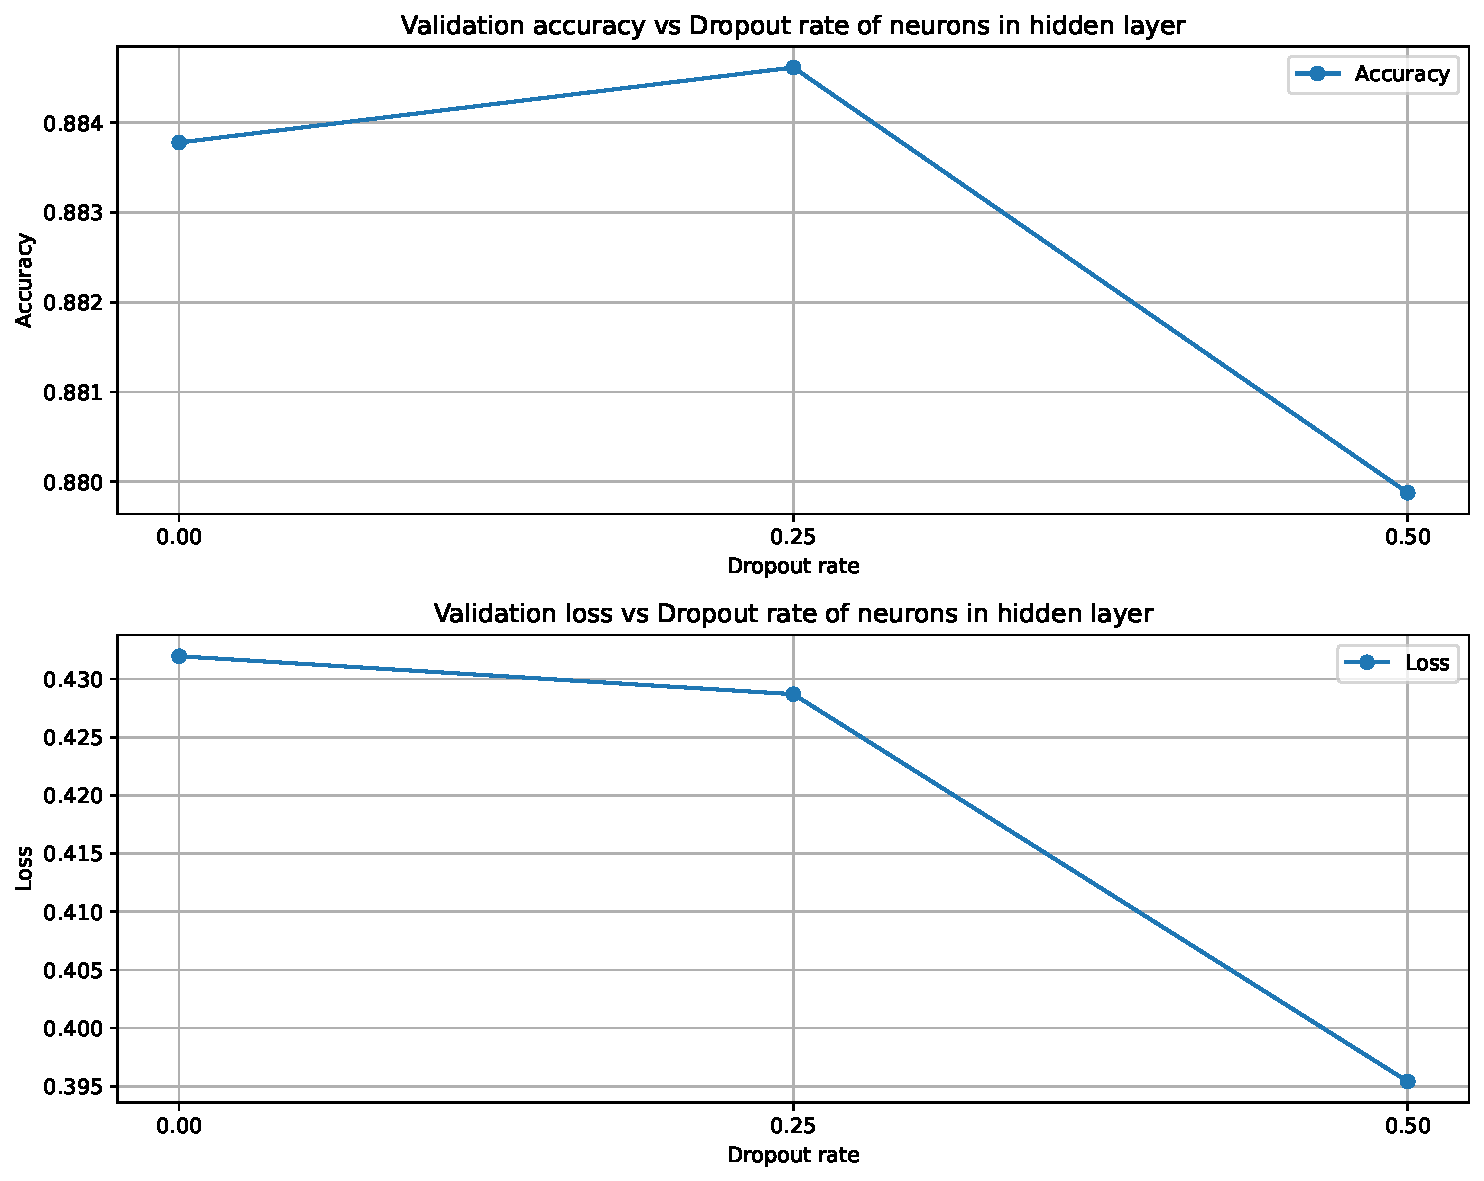
\includegraphics[width=0.75\linewidth]{../../plot/mlp/search_dropout}
\caption{Acurácia e perda com a variação da taxe de \textit{dropout} dos neurônios da camada intermediária.}
\label{fig:search_dropout}
\end{figure}

\subsubsection{Otimizador}

\begin{figure}[H]
	\centering
	\begin{subfigure}[H]{0.49\textwidth}
		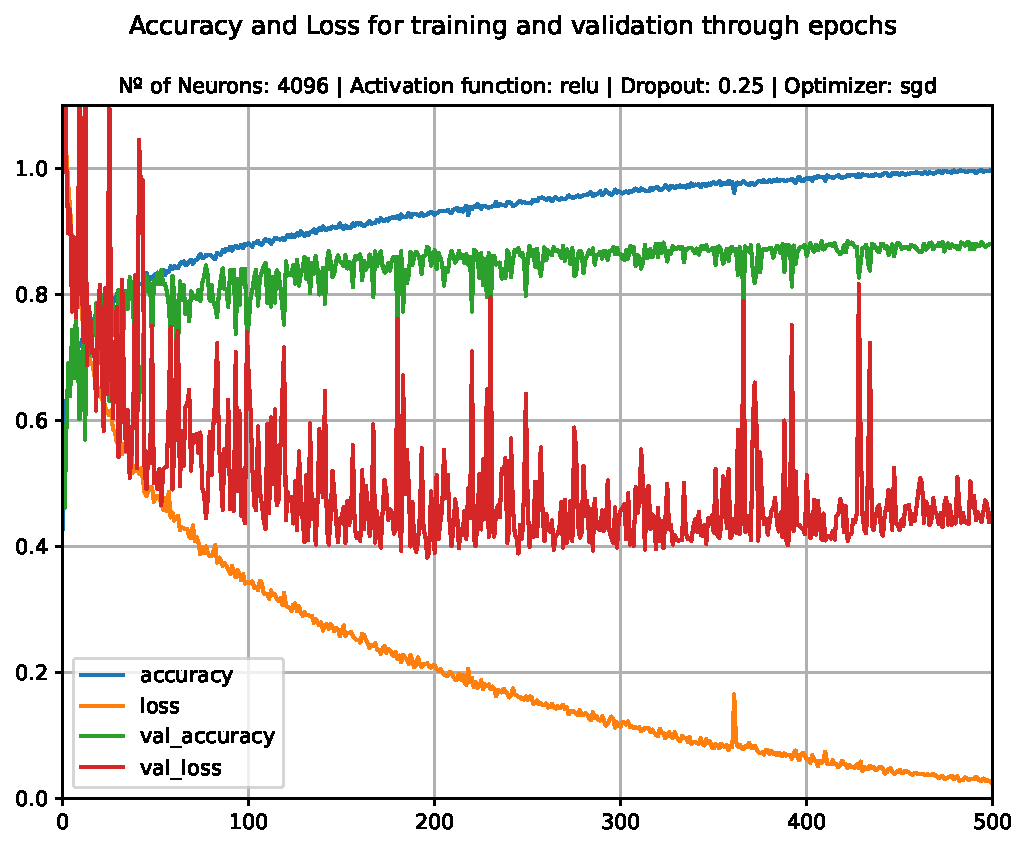
\includegraphics[width = \textwidth]{../../plot/mlp/mlp_4096_relu_0.25_sgd}
		\caption{ReLU.}
		\label{fig:mlp_4096_relu_0.0_sgd_opt}
	\end{subfigure}
	\begin{subfigure}[H]{0.49\textwidth}
		\centering
		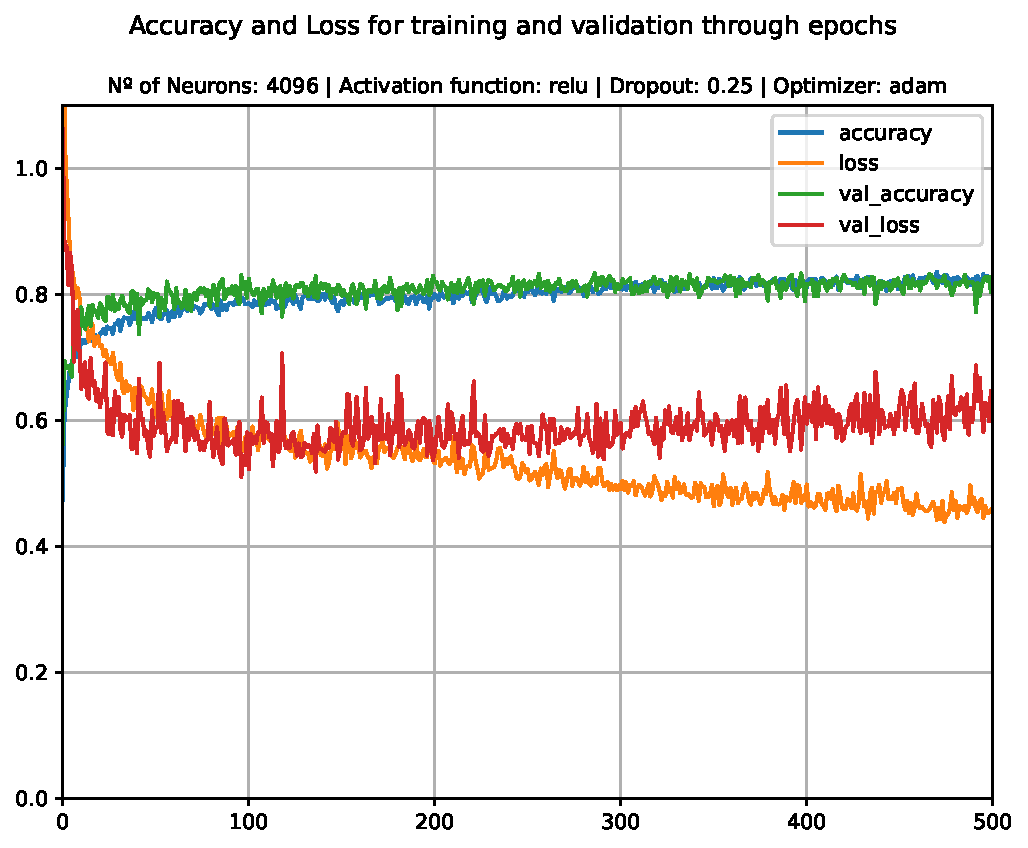
\includegraphics[width = \textwidth]{../../plot/mlp/mlp_4096_relu_0.25_adam}
		\caption{Sigmoide.}
		\label{fig:mlp_4096_relu_0.25_adam}
	\end{subfigure}
	\caption{Evolução da perda e acurácia de treinamento e validação com as épocas de treinamento para os otimizadores analisados.}
\end{figure}

\begin{figure}[H]
\centering
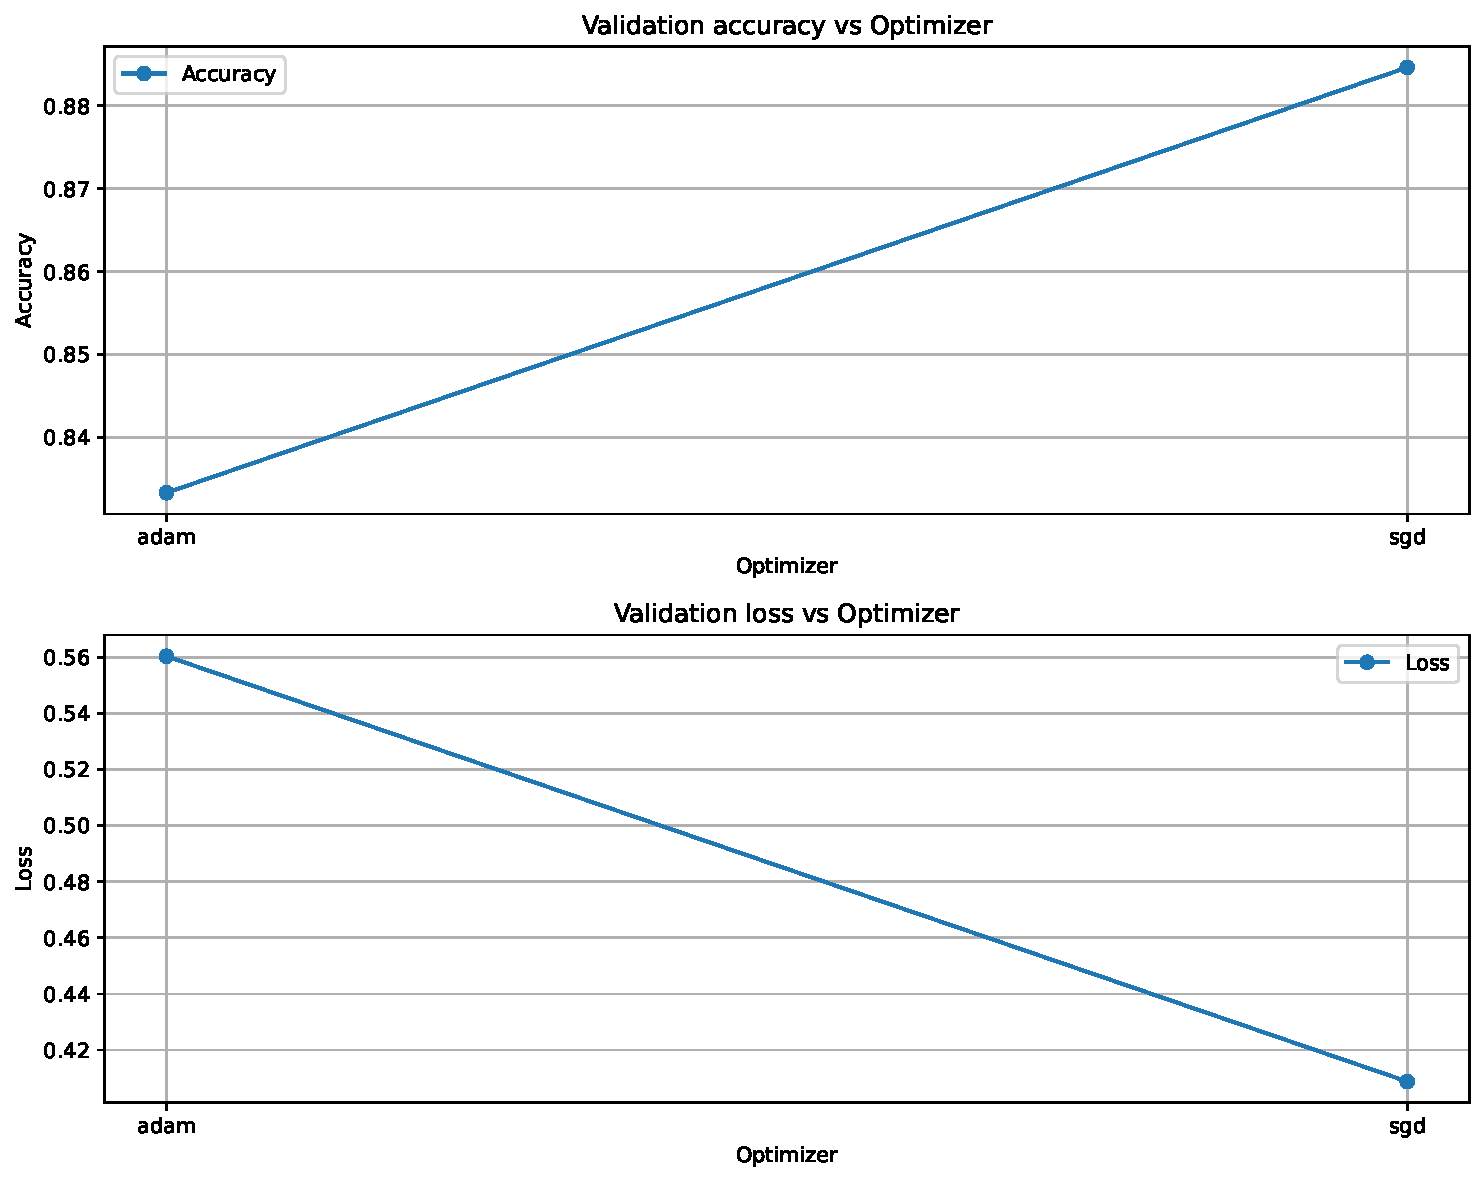
\includegraphics[width=0.75\linewidth]{../../plot/mlp/search_optimizer}
\caption{Acurácia e perda com a variação do algoritmo de otimização.}
\label{fig:search_optimizer}
\end{figure}

\subsection{Análise do melhor modelo}

\begin{equation}\label{eq:acc_MLP}
	Accuracy = 0.8705
\end{equation}

\begin{equation}\label{eq:ba_MLP}
	BA = 0.8437
\end{equation}


\begin{table}[H]
	\centering
	\begin{tabular}{c||c|c|c|c|c|c|c|c|}
		\cline{2-9}
		\textbf{}                        & \textbf{0} & \textbf{1} & \textbf{2} & \textbf{3} & \textbf{4} & \textbf{5} & \textbf{6} & \textbf{7} \\ \hline \hline
		\multicolumn{1}{|c||}{\textbf{0}} & 177        & 3          & 0          & 43         & 4          & 17         & 0          & 0          \\ \hline
		\multicolumn{1}{|c||}{\textbf{1}} & 1          & 613        & 0          & 3          & 1          & 0          & 6          & 0          \\ \hline
		\multicolumn{1}{|c||}{\textbf{2}} & 4          & 1          & 264        & 16         & 6          & 3          & 11         & 6          \\ \hline
		\multicolumn{1}{|c||}{\textbf{3}} & 34         & 26         & 3          & 447        & 5          & 32         & 32         & 0          \\ \hline
		\multicolumn{1}{|c||}{\textbf{4}} & 13         & 0          & 11         & 31         & 182        & 0          & 6          & 0          \\ \hline
		\multicolumn{1}{|c||}{5}          & 10         & 2          & 1          & 48         & 3          & 215        & 5          & 0          \\ \hline
		\multicolumn{1}{|c||}{\textbf{6}} & 0          & 22         & 5          & 22         & 2          & 2          & 611        & 2          \\ \hline
		\multicolumn{1}{|c||}{\textbf{7}} & 0          & 0          & 1          & 0          & 0          & 0          & 0          & 469        \\ \hline
	\end{tabular}
	\caption{Matriz de confusão do classificador baseado em MLP.}
	\label{tab:mc_MLP}
\end{table}

\begin{table}[H]
\centering
\begin{tabular}{c|c|c}
	\textbf{Classe} & \textbf{Precisão} & \textit{\textbf{Recall}} \\ \hline
	\textbf{0}     & 0.7254            & 0.7406                   \\
	\textbf{1}     & 0.9824            & 0.9190                   \\
	\textbf{2}     & 0.8489            & 0.9263                   \\
	\textbf{3}     & 0.7720            & 0.7328                   \\
	\textbf{4}     & 0.7490            & 0.8966                   \\
	\textbf{5}     & 0.7570            & 0.7993                   \\
	\textbf{6}     & 0.9174            & 0.9106                   \\
	\textbf{7}     & 0.9979            & 0.9832                  
\end{tabular}
\caption{Precisão e \textit{recall} por classe do classificador baseado em MLP.}
\label{tab:pr_MLP}
\end{table}

\subsubsection{Análise dos erros}

\begin{figure}[H]
\centering
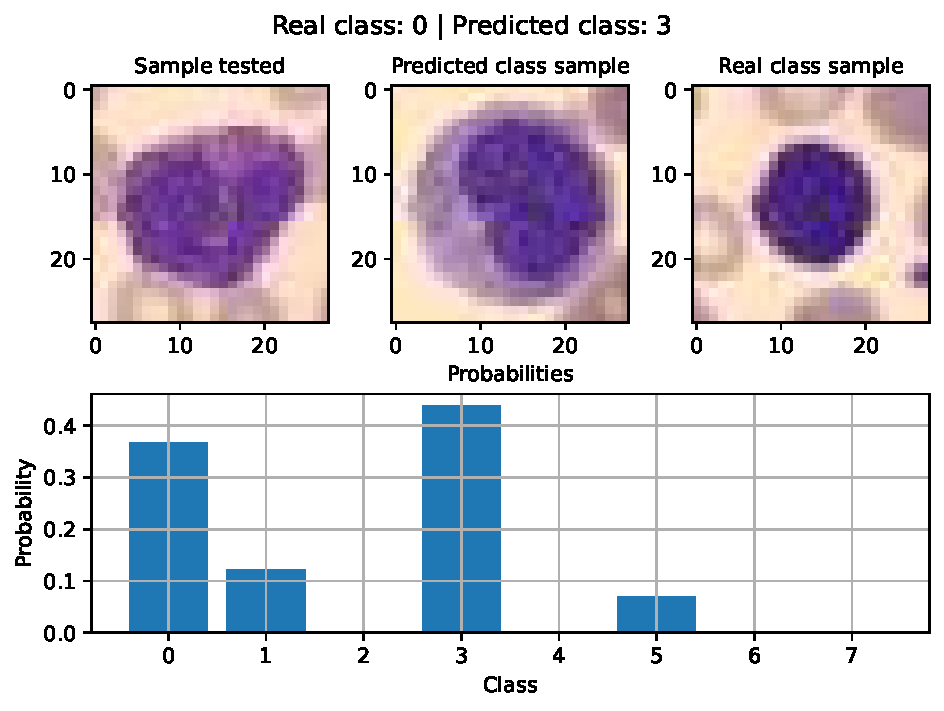
\includegraphics[width=0.75\linewidth]{../../plot/mlp/error_analyser_88}
\caption{Análise de um caso de erro de classificação.}
\label{fig:error_analyser_88}
\end{figure}

\begin{figure}[H]
\centering
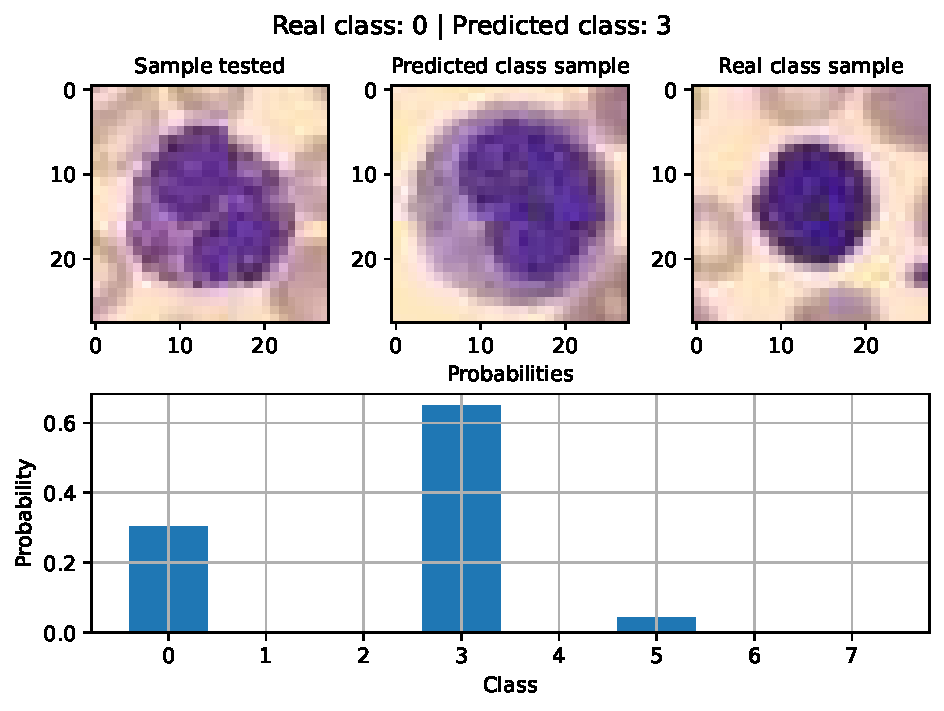
\includegraphics[width=0.75\linewidth]{../../plot/mlp/error_analyser_36}
\caption{Análise de um caso de erro de classificação.}
\label{fig:error_analyser_36}
\end{figure}

\begin{figure}[H]
\centering
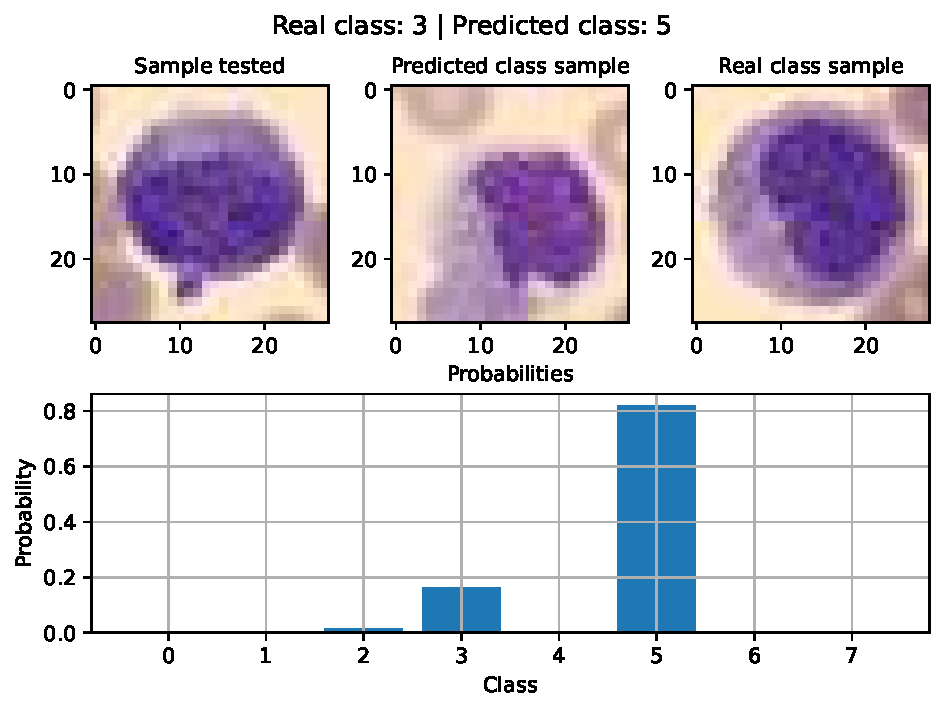
\includegraphics[width=0.75\linewidth]{../../plot/mlp/error_analyser_0}
\caption{Análise de um caso de erro de classificação.}
\label{fig:error_analyser_0}
\end{figure}

\begin{figure}[H]
\centering
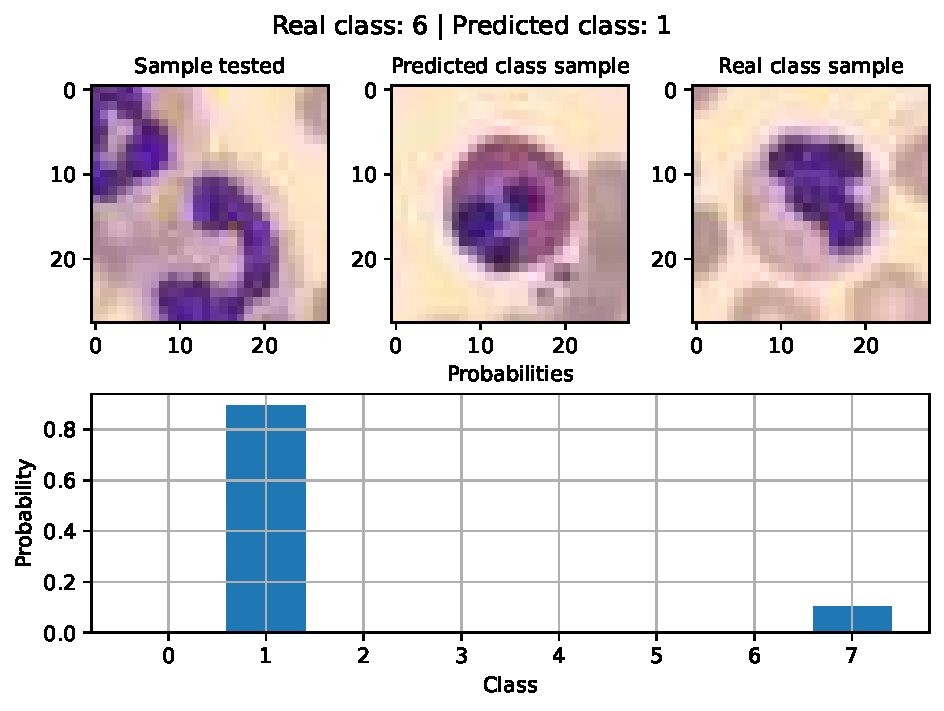
\includegraphics[width=0.75\linewidth]{../../plot/mlp/error_analyser_25}
\caption{Análise de um caso de erro de classificação.}
\label{fig:error_analyser_25}
\end{figure}

\begin{figure}[H]
\centering
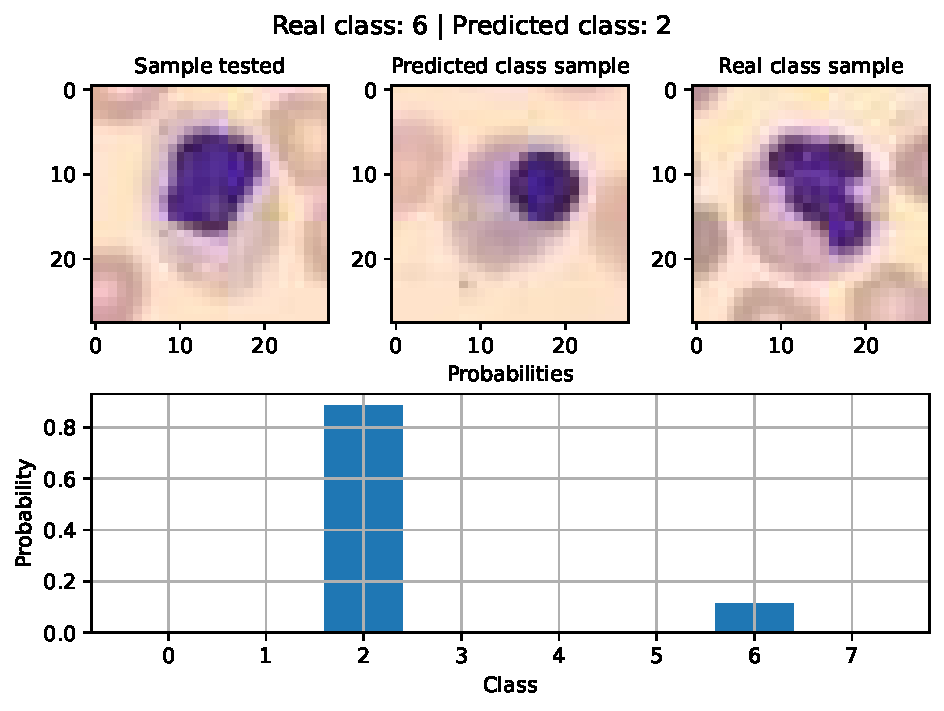
\includegraphics[width=0.75\linewidth]{../../plot/mlp/error_analyser_62}
\caption{Análise de um caso de erro de classificação.}
\label{fig:error_analyser_62}
\end{figure}

